% inspired from http://www.latex-community.org/forum/viewtopic.php?f=9&t=22340
\documentclass{article}

\usepackage{tikz}
\usetikzlibrary{arrows}
\usetikzlibrary{positioning}

\begin{document}

% DFS : exemple
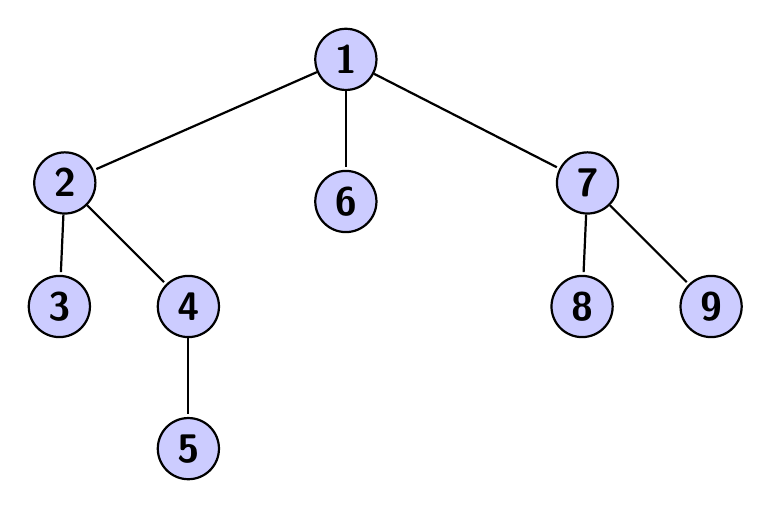
\begin{tikzpicture}[>=stealth', shorten >=1pt, auto, node distance = 3cm, thick, main node/.style = {circle, fill = blue!20, draw, font = \sffamily\Large\bfseries}]

	\node[main node] (1) {1};
	\node[main node] (2) [below left = 1cm and 3cm of 1] {2};
	\node[main node] (3) [below left = 1cm and -0.5cm of 2] {3};
	\node[main node] (4) [below right = 1cm and 1cm of 2] {4};
	\node[main node] (5) [below = 1cm of 4] {5};
	\node[main node] (6) [below = 1cm of 1] {6};
	\node[main node] (7) [below right = 1cm and 2.5cm of 1] {7};
	\node[main node] (8) [below left = 1cm and -0.5cm of 7] {8};
	\node[main node] (9) [below right = 1cm and 1cm of 7] {9};
	 
	\path[every node/.style = {font = \sffamily\small}]
	(1)	edge node {} (2)
		edge node {} (6)
		edge node {} (7)
	(2)	edge node {} (3)
		edge node {} (4)
	(4)	edge node {} (5)
	(7)	edge node {} (8)
		edge node {} (9);
\end{tikzpicture}

% BFS : pourquoi avoir besoin d'un BFS ?
\vspace{2cm}
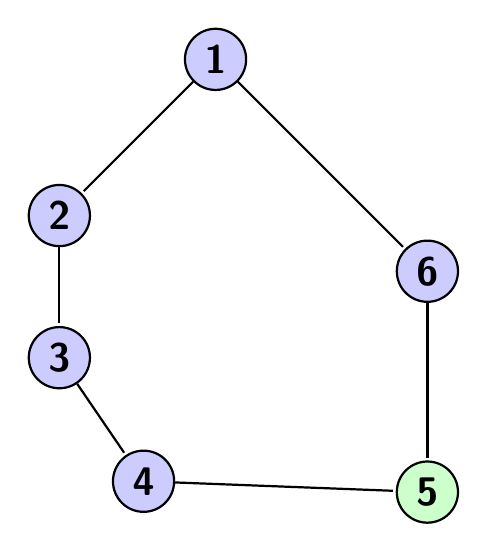
\begin{tikzpicture}[>=stealth', shorten >=1pt, auto, node distance = 3cm, thick, main node/.style = {circle, fill = blue!20, draw, font = \sffamily\Large\bfseries}]

	\node[main node] (1) {1};
	\node[main node] (2) [below left = 2cm of 1] {2};
	\node[main node] (3) [below = 1cm of 2] {3};
	\node[main node] (4) [below right = 1cm and 0.5cm of 3] {4};
	\node[main node] (6) [below right = of 1] {6};
	\node[main node, fill = green!20] (5) [below = 2cm of 6] {5};	
	
	 
	\path[every node/.style = {font = \sffamily\small}]
	(1)	edge node {} (2)
		edge node {} (6)
	(2)	edge node {} (3)
	(3) edge node {} (4)
	(4) edge node {} (5)
	(6) edge node {} (5);
\end{tikzpicture}

% BFS : exemple
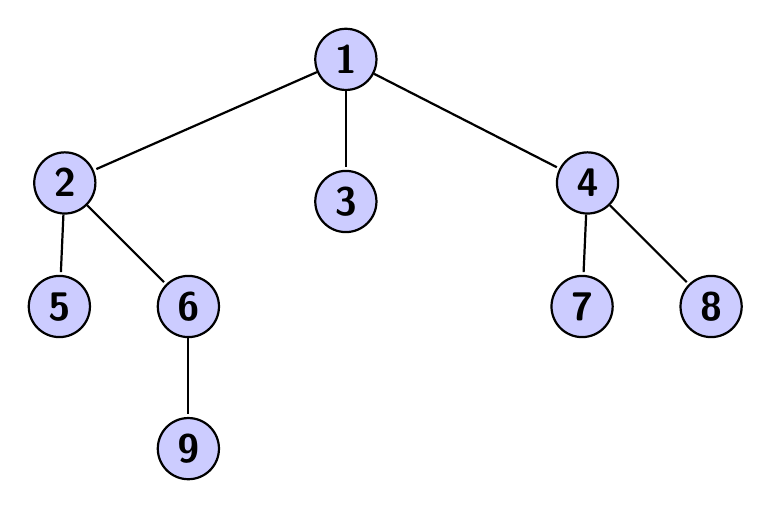
\begin{tikzpicture}[>=stealth', shorten >=1pt, auto, node distance = 3cm, thick, main node/.style = {circle, fill = blue!20, draw, font = \sffamily\Large\bfseries}]

	\node[main node] (1) {1};
	\node[main node] (2) [below left = 1cm and 3cm of 1] {2};
	\node[main node] (3) [below = 1cm of 1] {3};
	\node[main node] (4) [below right = 1cm and 2.5cm of 1] {4};
	\node[main node] (5) [below left = 1cm and -0.5cm of 2] {5};
	\node[main node] (6) [below right = 1cm and 1cm of 2] {6};
	\node[main node] (7) [below left = 1cm and -0.5cm of 4] {7};
	\node[main node] (8) [below right = 1cm and 1cm of 4] {8};
	\node[main node] (9) [below = 1cm of 6] {9};
	 
	\path[every node/.style = {font = \sffamily\small}]
	(1)	edge node {} (2)
		edge node {} (3)
		edge node {} (4)
	(2)	edge node {} (5)
		edge node {} (6)
	(4) edge node {} (7)
		edge node {} (8)
	(6)	edge node {} (9);
	
\end{tikzpicture}

\end{document}